\subsection{Elettrodo di prima specie}
Gli elettrodi visti finora appartengono a questa categoria. Essi sono metalli immersi in soluzioni dei loro ioni. Si fa ciò per raggiungere molto più velocemente l'equilibrio tra soluzione ed elettrodo, in quanto in acqua l'equilibrio è molto lento perché turbato dalla presenza degli ioni $\rm H_3O^+$ che competono assieme agli ioni liberati dal metallo nell'acqua per ritornare sull'elettrodo stesso.

L'elettrodo partecipa attivamente alla reazione, ossia è il metallo che libera ioni in soluzione, i quali lasciano elettroni sul metallo:

$$\ce{M <--> M^{n+} + ne^-}$$
\subsection{Elettrodo di seconda specie}
In questo caso il metallo è a contatto con un suo sale poco solubile, ad esempio argento Ag a contatto con cloruro di argento AgCl che è un sale insolubile. A sua volta il sale è a contatto con una soluzione di un sale (ovviamente solubile) che abbia l'anione in comune col sale poco solubile, quindi nel nostro esempio dovrà essere un sale che ha come anione ha lo ione cloruro, come il cloruro di potassio KCl. Un altro esempio è il mercurio Hg messo in contatto con un suo sale poco solubile che è il cloruro mercuroso $\rm Hg_2Cl_2$ (nota: i pedici non possono essere semplificati, tra poco vedremo perché), che a sua volta è a contatto con cloruro di potassio KCl.

Nello specifico, ciò che avviene nel primo esempio è che l'AgCl in minima parte si dissocia in $\rm Ag^+$ e $\rm Cl^-$

$$\ce{AgCl(s) <--> Ag^+ + Cl^-}$$

Se poi cediamo un elettrone ad $\rm Ag^+$, questo diventa $\rm Ag^0$, cioè argento metallico:

$$\ce{Ag^+ e^- <--> Ag}$$

In questo modo abbiamo ridotto l'argento.

La reazione totale allora sarà

$$\ce{AgCl(s) + e^- <--> Ag + Cl^-}$$
\subsection{Elettrodo di terza specie}
In esso un metallo nobile (cioè che non prende parte ai processi elettrolitici, funge solo da trasportatore di cariche) è immerso in una soluzione che contiene già stati ossidati e stati ridotti di un qualunque sistema redox.

Un esempio è un elettrodo di platino Pt che è un metallo nobile, immerso in una soluzione contenente un sale di ferro (II) e uno di ferro (III). Il platino fungerà solo da trasportatore di carica e lo stato ossidato e quello ridotto saranno rispettivamente lo stato ferrico e lo stato ferroso.

Consideriamo il permanganato $\rm MnO_4^-$. Esso in ambiente fortemente acido acquista 5 elettroni e diventa $\rm Mn^{2+}$, quindi $\rm MnO_4^-$ è lo stato ossidato e $\rm Mn^{2+}$ quello ridotto.

Va da ricordare che in ambiente fortemente acido ci sono ioni $\rm H_3O^+$, quindi la forma ossidata non è solo il permanganato ma anche gli ioni $\rm H_3O^+$. Anche in questo caso se usiamo il platino sarà un elettrodo di terza specie perché viene semplicemente immerso e funge da trasportatore di elettroni.

Un altro esempio è il chinidrone, una miscela di due polveri bianche, il chinone e l'idrochinone, che sono la forma ossidata e la forma ridotta. Sono utili perché permettono di misurare in maniera veloce il pH. Se immergiamo un filo di platino in una soluzione di questi composti, agirà come un elettrodo di terza specie.

\vspace{0.2cm}Scriviamo le equazioni di Nernst relative ai vari elettrodi:

\vspace{0.2cm} $\bullet$ \textbf{Elettrodo di prima specie}

$$\ce{Cu^{2+} + 2e^- <--> Cu} \quad E= E^0 + \frac{0.059}{2}\log \frac{a_{\text{Cu}^{2+}}}{a_{\text{Cu}}}$$

$$a_{\text{Cu}}=1 \implies E= E^0 + \frac{0.059}{2}\log a_{\text{Cu}^{2+}}$$

Questa sarà la d.d.p. di questo semielemento/elettrodo.

Va da ricordare che poi nei calcoli usiamo la concentrazione, non l'attività.

\vspace{0.2cm} $\bullet$ \textbf{Elettrodo di terza specie}

Per convenzione le reazioni si scrivono come riduzione, quindi

$$\rm Pt\,/\,Fe^{2+}, \; Fe^{3+} \implies \ce{Fe^{3+} + e^- <--> Fe^{2+}} $$

$$E = E^0 + \frac{0.059}{1} \log \frac{a_{\text{Fe}^{3+}}}{a_{\text{Fe}^{2+}}}$$

$$\rm Pt\,/\,Mn^{2+}, \; MnO_4^- \implies \ce{MnO_4^- + 8H^+ + 5e^- <--> Mn^{2+} + 4H_2O} $$

Questa è la semi-reazione relativa al permanganato. La d.d.p. relativa ad un filo di platino immerso in una soluzione di $\rm MnO_4^-$ e $\rm Mn^{2+}$ sarà

$$E = E^0 + \frac{0.059}{5} \log \frac{a_{\text{MnO}_4^-} \cdot a^8_{\text{H}^+}}{a_{\text{Mn}^{2+}}}$$

Attenzione! Abbiamo scritto d.d.p. ma è corretto dire il potenziale.
\subsection{Elettrodo normale standard ad idrogeno}
Finora non siamo stati in grado di misurare i potenziali. Per fare ciò si sceglie un elettrodo e si usa come riferimento. Ad esso si assegna un potenziale arbitrario (nel caso particolare si è assegnato valore zero) e si usa questo come secondo elettrodo per fare le misure di tutti i potenziali di qualunque altro elettrodo.

Quindi la d.d.p. tra elettrodo e soluzione non è misurabile perché dovremmo introdurre un tester che farebbe da secondo elettrodo.

Come riferimento si è scelto l'elettrodo normale standard a idrogeno:
\comment{
\begin{minipage}{0.55\textwidth}
    \begin{figure}[H]
        \centering
        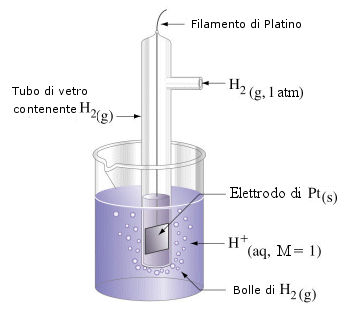
\includegraphics[width=8cm]{immagini/Elettrodo_a_idrogeno.png}
    \end{figure}
\end{minipage}
\begin{minipage}{0.45\textwidth}
    \vspace{0.7cm}Immaginiamo di avere un beker contenente una soluzione 1-molare di HCl in cui mettiamo un filo di platino saldato ad una lamina di platino, la quale in superficie è ricoperta di una polvere finissima di platino. Tale oggetto si chiama \textit{platino platinato}. Viene rivestito per aumentare la superficie di disposizione, perché si conta la superficie di ogni granello. Facciamo gorgogliare (quindi sotto la lamina) l'idrogeno che è un gas. Esso gorgogliando aderisce alla superficie della lamina, in quanto i grani finissimi di platino che ricoprono la lamina di platino fungono da supporto per le bollicine di idrogeno che vanno ad aderire sulla lamina.
\end{minipage}
}

\begin{figure}[H]
    \centering
    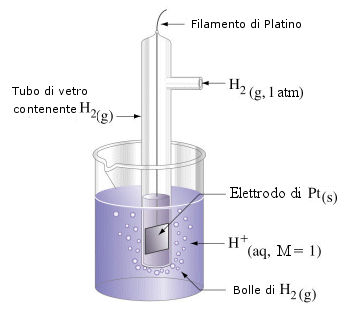
\includegraphics[width=9cm]{immagini/Elettrodo_a_idrogeno.png}
\end{figure}

Immaginiamo di avere un beker contenente una soluzione 1-molare di HCl in cui mettiamo un filo di platino saldato ad una lamina di platino, la quale in superficie è ricoperta di una polvere finissima di platino. Tale oggetto si chiama \textit{platino platinato}. Viene rivestito per aumentare la superficie di disposizione, perché si conta la superficie di ogni granello. Facciamo gorgogliare (quindi sotto la lamina) l'idrogeno che è un gas. Esso gorgogliando aderisce alla superficie della lamina, in quanto i grani finissimi di platino che ricoprono la lamina di platino fungono da supporto per le bollicine di idrogeno che vanno ad aderire sulla lamina.

\vspace{0.2cm}Perché si chiama standard?

Dato che abbiamo idrogeno che gorgoglia alla pressione di 1 atm e a 25° C, siamo in condizioni standard.

Perché si chiama normale?

La normalità è definita come il numero di equivalenti su un litro di soluzione. Nel caso dell'acido cloridrico che libera un solo protone, molarità e normalità coincidono perchè coincidono moli ed equivalenti, per cui concentrazione 1-molare significa anche concentrazione 1-normale in questo caso.

La reazione che avviene è

$$\ce{2H_3O^+ + 2e^- <--> 2H_2O + H_2}$$

Può anche essere immaginata come due ioni $\rm H^+$ che acquistano 2 elettroni e formano $\rm H_2$. In entrambi i casi è una riduzione.

Il potenziale di questa reazione è

$$E = E^0 + \frac{0.059}{2} \log \frac{a^2_{\text{H}_3\text{O}^+}}{a_{\text{H}_2}}$$

L'attività di un gas che gorgoglia a pressione atmosferica è pari a 1, per cui

$$E = E^0 + 0.059 \log a_{\text{H}_3\text{O}^+}$$

L'attività degli ioni $\rm H_3O^+$ è pari a 1 (perché 1-molare), quindi il logaritmo si azzera e otteniamo $E=E^0$. In queste condizioni il potenziale dell'elettrodo normale standard ad idrogeno è pari a $0.000 V$.

Dunque tutte le volte che vogliamo misurare il potenziale di un qualunque elettrodo, dato che per fare una misura serve un secondo elettrodo useremo questo come riferimento. Ne segue che tutti i potenziali che misureremo saranno dei \textbf{potenziali normali standard} $E^0$.

In realtà è difficoltoso usare questo elettrodo, perché si deve avere una bombola che eroghi costantemente idrogeno ad 1 atm esatto. Pertanto questo elettrodo è il riferimento teorico ma non quello che si usa praticamente.
\subsection{Elettrodo a calomelano saturo}
\E un elettrodo a mercurio ed è quello che poi viene usato nella pratica. Si chiama così perché è presente il composto $\rm Hg_2Cl_2$, che si chiama calomelano.

Perché non possiamo semplificare i pedici in $\rm Hg_2Cl_2$?

Perché lo ione in soluzione non è $\rm Hg^+$ ma è $\rm Hg_2^{2+}$, cioè ci sono due ioni che stanno assieme formando un dimero.

\begin{minipage}{0.35\textwidth}
    \begin{figure}[H]
        \centering
        \includegraphics[width=5cm]{immagini/Elettrodo_a_calomelano.png}
    \end{figure}
\end{minipage}
\begin{minipage}{0.63\textwidth}
    \vspace{0.4cm}Tale elettrodo è costituito da un bulbo di vetro in cui abbiamo mercurio Hg liquido. Per realizzare il contatto elettrico è saldato al bulbo un filo di platino che tocca il mercurio dentro ed esce fuori. In questo modo il contatto elettrico è assicurato sia dentro che fuori.

    Il metallo deve essere a contatto con una soluzione di un suo sale poco solubile, che è l'$\rm Hg_2Cl_2$. Questo a sua volta è a contatto con un sale con cui ha in comune l'anione, che è il KCl. Quest'ultimo si trova nella gelatina di agar-agar che costituisce il ponte salino. In questo modo in questo elettrodo abbiamo entrambi i collegamenti: il filo metallico e il ponte salino per collegarlo ad un'altra soluzione.
\end{minipage}

\vspace{0.4cm}Ciò che avviene è che l'$\rm Hg_2Cl_2$ si dissocia in $\rm Hg_2^{2+}$ più due ioni cloruro $\rm Cl^-$:

$$\ce{Hg_2Cl_2(s) <--> Hg_2^{2+} + 2Cl^-}$$

Se poi ad $\rm Hg_2^{2+}$ forniamo due elettroni otteniamo due atomi di mercurio:

$$\ce{ Hg_2^{2+} + 2e^- <--> 2Hg}$$

Globalmente la reazione sarà

$$\ce{Hg_2Cl_2(s) + 2e^- <--> 2Hg + 2Cl^-}$$

Il potenziale di questa reazione sarà

$$E=E^0 + \frac{0.059}{2} \log \frac{a_{\text{Hg}_2\text{Cl}_2(s)}}{a^2_{\text{Hg}} \cdot a^2_{\text{Cl}^-}}$$

Il mercurio è un metallo puro, quindi la sua attività è unitaria. Il calomelano saturo è un solido puro e l'attività dei solidi è sempre unitaria. Quindi resta

$$E=E^0 + \frac{0.059}{2} \log \frac{1}{a^2_{\text{Cl}^-}}\quad
\implies E=E^0 + \frac{0.059}{2} \log a^{-2}_{\text{Cl}^-}$$

$$\implies E=E^0 - \frac{0.059}{2} \cdot 2 \log a_{\text{Cl}^-}
\quad
\implies E=E^0 - 0.059 \log a_{\text{Cl}^-}$$

Il potenziale di Nernst di questo elettrodo dipenderà allora dalla concentrazione dello ione cloruro (infatti se misuriamo una d.d.p. tra questo elettrodo e quello normale standard a idrogeno, dato che per definzione il potenziale del secondo è pari a zero, quello che misuriamo è imputabile tutto a questo elettrodo). Abbiamo così scoperto un modo per misurare la concentrazione di uno ione. Se ad esempio vogliamo sapere se dell'acqua è potabile, misurando la d.d.p. è possibile calcolare la concentrazione degli ioni $\rm Cl^-$.

Con questo metodo siamo in grado di costruire una reazione che ci permette, tramite una misura di d.d.p.\,, di quantificare la presenza (cioè la concentrazione) di uno ione, e ciò per qualunque specie chimica. Gli oggetti che permettono tali misure si chiamano \textit{elettrodi ion-selettivi}. Essi sono sensori elettro-chimici, che una volta immersi leggono la concentrazione dello ione. Ce n'è uno specifico per ogni ione.

Quindi ciò che si deve fare è andare a cercare la reazione giusta, quella più adatta, poi costruiamo un elettrodo il cui potenziale dipenda, tramite questa reazione, da ciò che vogliamo misurare.

La maggior parte dei sensori usa l'elettrochimica.

Nel nostro esempio tale elettrodo ci permette di misurare la concentrazione del KCl. Se questo dovesse essere 1-molare, $a_{\text{Cl}^-}=1$ e allora diventa $E=E^0=0.268 V$

\vspace{0.2cm}Nota: nelle misure di potenziale si usano 3 cifre dopo la virgola.

\vspace{0.2cm}Quindi l'elettrodo di riferimento è quello normale standard a idrogeno, ma quello che poi si usa è l'elettrodo a calomelano saturo che, se costruito in modo tale che l'attività dello ione cloruro sia unitaria avrà un potenziale pari a quello sopra. Esso è semplice da usare perché per toccare qualunque cosa c'è solo un filo di platino e nella sua struttura è già incluso il ponte salino.

Quello che si fa nella pratica è immergere il ponte salino nel beker contenente l'altro elettrodo e col filo di platino tocchiamo il tester. A questo punto poggiamo un puntale sul filo di platino e l'altro sul secondo elettrodo.

Inizialmente non si era pensato di mettere il filo di platino. Al suo posto il bulbo aveva un piccolo foro da cui il mercurio gocciolava lentamente. La goccia che stava per cadere era a contatto con il mercurio dentro e con la soluzione esterna. Tale sistema si chiamava \textit{elettrodo a goccia di mercurio}. La limitazione era che il mercurio si esauriva, quindi si è messo il filo di platino per mantenere il contatto.
\subsection{Elettrodo d'argento}
Simile a quello a calomelano, in esso abbiamo un filo di argento Ag che è a contatto col cloruro di argento, il quale a sua volta è a contatto con cloruro di potassio. La reazione che avviene è
$$\ce{AgCl + 1e^- <--> Ag + Cl^-}$$
Il potenziale sarà
$$E = E^0 -0.059 \log a_{\text{Cl}^-}$$

Anche questo è un elettrodo il cui potenziale dipende dalla concentrazione degli ioni cloruro.

Se questa concentrazione è pari a 1 il potenziale sarà $E=0.2355 V$
\subsection{Elettrodo al chinidrone}
Il chinidrone è formato da benzochinone e idrochinone, forma ossidata e forma ridotta:

\begin{center}
    \begin{tabular}{p{2.4cm}p{2.5cm}p{2.1cm}p{2cm}}
    \chemfig{*6(-(=O)-=-(=O)-=)} & \vspace{-0.8cm}$\rm + \; 2H^+ \; + \; 2e^-$ & \vspace{-0.9cm} \schemestart \arrow{<=>}      \schemestop &
    \chemfig{*6(=(-OH)-=-(-OH)=-)}\\
    \vspace{0.2cm}\hspace{-0.1cm}Benzochinone & & & \vspace{0.2cm}Idrochinone
    \end{tabular}
\end{center}

Esse sono due polveri bianche che per questo tipo di misure vengono vendute già mescolate insieme in quantità equimolari.

Il potenziale sarà

$$E = E^0 + \frac{0.059}{2} \log \frac{a_{\text{Benzochinone}} \cdot a^2_{\text{H}^+}}{a_{\text{Idrochinone}}}$$

Essendo equimolari, qualunque sia il volume di chinidrone preso avremo le stesse moli di benzochinone e idrochinone, per cui la concentrazione sarà identica, quindi le loro attività si semplificano qualunque sia il volume. Avremo allora

$$E = E^0 + 0.059 \log a_{\text{H}^+}$$

Il logaritmo ricorda molto il pH, che può essere calcolato se scriviamo $E$ come

$$E = E^0 - 0.059 \log \left( \frac{1}{a_{\text{H}^+}} \right)$$

\vspace{1cm}Vediamo adesso una tabella di valori dei potenziali per i vari elettrodi. In essa abbiamo valori di potenziali standard sia negativi che positivi. Il riferimento è l'elettrodo a idrogeno, per il quale la reazione di riduzione ha potenziale di riduzione $E^0$ pari a 0. 

\begin{center}
    \scriptsize\begin{tabular}{|ll|ll|}
        \hline
        &&&\\
        Reazione & $E^0 \; (V)$ & Reazione & $E^0 \; (V)$\\
        &&&\\
        \hline
        &&&\\
        \ce{Li^+ + e^- <--> Li} & -3.045 & \ce{S_4O_6^{2-} <--> 2S_2O_3^{2-}} & 0.10\\[0.7ex]
        \ce{K^+ + e^- <--> K} & -3.924 & \ce{S + 2H_3O^+ + 2e^- <--> H_2S + 2H_2O} & 0.14\\[0.7ex]
        \ce{Ca^{2+} + 2e <--> Ca} & -2.76 & \ce{Sn^{4+} 2e^- <--> Sn^{2+} (HCl \; 1F)} & 0.15\\[0.7ex]
        \ce{Na^+ + e^- <--> Na} & -2.7109 & \ce{Cu^{2+} + e^- <--> Cu^+} & 0.158\\[0.7ex]
        \ce{Mg^{2+} + 2e^- <--> Mg} & -2.375 & \ce{Hg_2Cl_2 + 2e^- <--> 2Hg + 2Cl^-} & 0.2682\\[0.7ex]
        \ce{H_3O^+ + e^- <--> H_2O + H} & -2.10 & \ce{Cu^{2+} + 2e^- <--> Cu} & 0.337\\[0.7ex]
        \ce{Al^{3+} + 3e^- <--> Al} & -1.71 & \ce{O_2 + 2H_2O + 4e^- <--> 4OH^-} & 0.401\\[0.7ex]
        \ce{Ti^{2+} + 2e^- <--> Ti} & -1.63 & \ce{Cu^+ + e^- <--> Cu} & 0.521 \\[0.7ex]
        \ce{ZnO_2^{2-} + 2H_2O + 2e^- <--> Zn + 4OH^-} & -1.22 & \ce{I_2 + 2e^- <--> 2I^-} & 0.536 \\[0.7ex]
        \ce{Mn^{2+} + 2e^- <--> Mn} & -1.03 & \ce{O_2 + 2H_3O^+ + 2e^- <--> H_2O_2 + 2H_2O} & 0.682 \\[0.7ex]
        \ce{2H_2O + 2e^- <--> H_2 + 2OH^-} & -0.828 & \ce{Fe^{3+} + e^- <--> Fe^{2+}} & 0.771\\[0.7ex]
        \ce{Zn^{2+} + 2e^- <--> Zn} & -0.7628 & \ce{Hg_2^{2+} + 2e^- <--> 2Hg} & 0.7961 \\[0.7ex]
        \ce{Cr^{3+} + 3e^- <--> Cr} & -0.74 & \ce{Ag + e^- <--> Ag} & 0.7996\\[0.7ex]
        \ce{Te + 2H_3O^+ +2e^- <--> H_2Te + 2H_2O} & -0.72 & \ce{2NO_3^- + 4H_3O^+ + 2e^- <--> N_2O_4 + 6H_2O} & 0.80\\[0.7ex]
        \ce{As + 3H_3O^+ + 3e^- <--> AsH_3 + 3H_2O} & -0.60& \ce{NO_3^- + 3H_3O^+ + 2e^- <--> HNO_2 + 4H_2O} & 0.94\\[0.7ex]
        \ce{Cr^{2+} + 2e^- <--> Cr} & -0.557 & \ce{NO_3^- + 4H_3O^+ + 3e^- <--> NO + 6H_2O} & 0.96\\[0.7ex]
        \ce{H_3PO_2 + H_3O^+ + e^- <--> P + 3H_2O} & -0.51 & \ce{Br_2 + 2e^- <--> 2Br^-} & 1.087\\[0.7ex]
        \ce{Fe^{2+} + 2e^- <--> Fe} & -0.409& \ce{Pt^{2+} + 2e^- <--> Pt} & 1.2\\[0.7ex]
        \ce{Cr^{3+} + e^- <--> Cr^{2+}} & -0.41 & \ce{MnO_2 + 4H_3O^+ + 4e^- <--> Mn^{2+} + 6H_2O} & 1.21\\[0.7ex]
        \ce{Cd^{2+} + 2e^- <--> Cd} & -0.4026 & \ce{O_2 + 4H_3O^+ + 4e^- <--> 6H_2O} & 1.229\\[0.7ex]
        \ce{Se + 2H_3O^+ + 2e^- <--> H_2Se + 2H_2O} & -0.40 & \ce{Cr_2O_7^{2-} + 14H_3O^+ + 6e^- <--> 2Cr^{3+} + 21H_2O} & 1.33 \\[0.7ex]
        \ce{Tl^+ + e^- <--> Tl} & -0.3363 & \ce{Cl_2 + 2e^- <--> 2Cl^-} & 1.358 \\[0.7ex]
        \ce{Co^{2+} +2e^- <--> Co} & -0.277 & \ce{ClO_3^- + 6H_3O^+ + 6e^- <--> 6Cl^- + 9H_2O} & 1.45\\[0.7ex]
        \ce{Ni^{2+} + 2e^- <--> Ni} & -0.230 & \ce{PbO_2 + 4H_3O^+ + 2e^- <--> Pb^{2+} + 6H_2O} & 1.455\\[0.7ex]
        \ce{N_2 + 5H_3O^+ -2e^- <--> N_2H_5^+ + 5H_2O} & -0.23 & \ce{MnO_4^- + 8H_3O^+ +5e^- <--> Mn^{2+} + 12H_2O} & 1.50\\[0.7ex]
        \ce{Sn^{2+} + 2e^- <--> Sn} & -0-1364 & \ce{HClO + H_3O^+ + e^- <--> \frac{1}{2} Cl_2 + 2H_2O} & 1.63\\[0.7ex]
        \ce{Pb + 2e^- <--> Pb} & -0.1263 & \ce{H_2O_2 + 2H_3O^+ + 2e^- <--> 4H_2O} & 1.776\\[0.7ex]
        \ce{2H_3O^+ + 2e^- <--> H_2 + 2H_2O} & 0.000 & \ce{Co^{3+} + e^- <--> Co^{2+} (HNO_3 \; 3F)} & 1.842\\[0.7ex]
        \ce{NO_3^- + H_2O + 2e^- <--> NO_2^- + 2OH^-} & 0.0 & \ce{F_2 + 2e <--> 2F^-} & 2.87\\[0.7ex]
        \hline
    \end{tabular}
\end{center}
\normalsize

\vspace{0.2cm}Riprendiamo il primo esempio di pila: se immergiamo un filo di rame in acqua, esso libera ioni e si carica negativamente. Analogamente avviene con un filo di zinco. Tuttavia uno dei due elementi libera molti più ioni di quanti ne liberi l'altro, e di conseguenza si caricherà molto più negativamente. Se allora li accoppiamo, diremo che quello più negativo sarà il polo negativo e l'altro il polo positivo, in quanto da un punto di vista dell'energia potenziale gli elettroni fluiranno da quello più carico negativamente a quello meno carico negativamente.

Dal concetto di elettronegatività sappiamo poi che ci sono elementi a bassa elettronegatività che tendono a cedere elettroni e elementi ad alta elettronegatività che tendono invece ad acquistarli. Se allora avessimo, ad esempio, un filo di sodio e lo immergessimo in acqua, questo libererebbe ioni e qualora fosse possibile (non lo è perché esplode) si caricherebbe negativamente ciò che non si scioglie (il filo di sodio si scioglie subito, liberando idrogeno) di una quantità enorme di elettroni, ed infatti troviamo il sodio tra gli elettrodi a potenziale più negativo insieme a litio, potassio e calcio perché liberano molti ioni.

Sotto l'idrogeno abbiamo invece potenziali positivi, e il più alto è quello dato dalla riduzione del fluoro.

Va da notare che i valori sono quelli di $E^0$ perché se la concentrazione è unitaria il logaritmo si annulla e ciò che si misura è proprio $E^0$. Ricordiamo poi che è possibile misurare questo usando come riferimento l'elettrodo standard a idrogeno, in modo tale che il potenziale misurato sia imputabile tutto all'elettrodo.

L'importanza di costruire una scala di valori è che se vogliamo calcolare il potenziale di un elettrodo dobbiamo innanzitutto conoscere il suo $E^0$, perché in funzione del suo valore potremo prevedere se effettivamente le reazioni di riduzione avvengono. Infatti un semielemento si riduce tanto più facilmente quanto maggiore è il valore del suo potenziale normale standard. Quindi se abbiamo un insieme di reazioni, avverrà quella la cui specie che si riduce ha il potenziale più alto.

Se ad esempio avessimo cloruro di sodio in acqua, applicando una d.d.p. e immergendo due fili di platino, non potremo mai ridurre il sodio in acqua perché in acqua abbiamo ioni $\rm H_3O^+$ che possono ridursi dando $\rm H_2O$ e il loro potenziale è zero, mentre il potenziale di riduzione del sodio è -2.7109, che è più basso. Ne segue che se facessimo l'elettrolisi di una soluzione di NaCl svilupperemmo idrogeno e non il sodio. Pertanto dal punto di vista termodinamico in acqua non possiamo ridurre nessuno degli elettrodi che stanno sopra l'idrogeno, perché hanno tutti potenziale negativo, quindi anziché loro sarà l'idrogeno a ridursi.

\vspace{0.2cm}Quindi si riducono le speci che hanno il potenziale standard maggiore. Tutti gli elementi a potenziale negativo non vedranno mai sviluppata la loro riduzione in soluzione, al loro posto sarà lo ione $\rm H^+$ a ridursi in idrogeno: \ce{2H^+ + 2e^- <--> H_2}.

In generale quindi possiamo scrivere una redox, ma non è detto che avvenga.

\vspace{0.2cm}\textbf{ES.1}
$$\ce{2Fe^{2+} + Sn^{4+} <--> Sn^{2+} + 2Fe^{3+}}$$

In questa reazione quello che pensiamo che avvenga è che lo ione ferroso $\rm Fe^{2+}$ liberi un elettrone e lo catturi lo stagno, il quale esiste in stato di ossidazione +2 e +4, quindi vuole 2 elettroni per passare da $\rm Sn^{4+}$ a $\rm Sn^{2+}$. Dato che nel passaggio in ione ferrico $\rm Fe^{+3}$ il ferro libera un solo elettrone ci serviranno due ioni $\rm Fe^{2+}$, che libereranno 2 elettroni i quali verranno catturati da uno ione $\rm Sn^{2+}$. Per vedere se tale reazione avviene, andiamo a vedere gli $E^0$ delle riduzioni di $\rm Sn^{4+}$ a $\rm Sn^{2+}$ e di $\rm Fe^{+3}$ a $\rm Fe^{2+}$:

$$E_0 \quad \text{Sn}^{4+}/ \, \text{Sn}^{2+}=0.15 V$$

\vspace{-0.3cm}$$E_0 \quad \text{Fe}^{3+}/ \, \text{Fe}^{2+}=0.77 V$$

Nella reazione è lo stagno a ridursi da +4 a +2, ma il potenziale della coppia dello stagno è minore di quello del ferro che è la specie che si ossida. Ne segue che questa reazione non avviene, anzi avviene la reazione opposta:

$$\ce{Sn^{2+} + 2Fe^{3+} <--> Sn^{4+} + 2Fe^{2+}}$$

\textbf{ES.2}

$$\ce{Fe +2H_3O^+ -> Fe^{2+}(aq) + 2H_2O + H_2}$$

Il ferro in acqua arrugginisce in quanto il $\rm Fe^0$ libera 2 elettroni e diventa $\rm Fe^{2+}$. Questi due elettroni vengono catturati da due ioni $\rm H^+$ che diventano $\rm H_2$. Il potenziale dell'idrogeno è zero, ed è la specie che si sta riducendo: da $\rm 2H^+$ a $\rm H_2$, mentre il potenziale di riduzione del ferro è -0.41V. Dato che è minore, la reazione avviene e il ferro in acqua arrugginisce.

\vspace{0.2cm}\textbf{ES.3}

$$\ce{Cu +2H_3O^+ -> Cu^{2+}(aq) + 2H_2O + H_2}$$

Il rame in acqua si scioglie e dà $\rm Cu^{2+}$ liberando due elettroni, i quali vengono presi da due ioni $\rm H^+$ che diventano $\rm H_2$.

Il potenziale dell'idrogeno è zero, quello della riduzione del rame è 0.337 V. Essendo più alto il potenziale delle specie che si ossida, questa reazione non può avvenire. Ecco perché i fili di rame possono essere lasciati scoperti, perché non si scioglie.

\subsubsection{Excursus: la placcatura}
Placcare un oggetto in un certo metallo significa prendere tale oggetto, immergerlo in una soluzione di un sale del metallo con cui vogliamo realizzare la placcatura (ad esempio per gli oggetti placcati in argento si usa il nitrato d'argento) e a questa applichiamo una d.d.p. in modo tale che il metallo si depositi come un film sottile omogeneo.

Quali metalli possiamo far depositare in acqua? Tutti quelli che hanno il potenziale maggiore di zero, perché altrimenti anziché ridursi il metallo gli elettroni saranno presi dall'idrogeno piuttosto che dagli ioni metallici.

\subsection{Pile chimiche (schematismo)}
\begin{center}
    \begin{tabular}{p{2cm}|p{2cm}||p{2cm}|p{2cm}}
        \vspace{0.3cm}elettrodo 1 & soluzione 1 & soluzione 2 & \vspace{0.3cm}elettrodo 2\\
        & attività 1 & attività 2 &
    \end{tabular}
\end{center}

In questo schema la doppia linea indica un ponte salino, mentre la linea singola si utilizza per separare sostanze in fase diverse nella stessa soluzione.

\vspace{0.2cm}\textbf{ES.1}
\begin{center}
    \begin{tabular}{p{2.3cm}|p{2cm}||p{1.8cm}|p{2cm}}
        Pt($\rm H_2$) & $\rm H_3O^+$ & $\rm Ag^+$ & Ag\\[0.5ex]
        P$\rm _{H_2}$=1 atm & $a_{\text{H}_3\text{O}^+}=1$ & $a_{\text{Ag}^+}=x$&\\[0.5ex]
    \end{tabular}
\end{center}

Abbiamo un filo di platino e uno di argento.

Il filo di argento è immerso in una soluzione di un sale di argento, quello di platino in una soluzione di ioni $\rm H_3O^+$ (è l'elettrodo normale standard ad idrogeno in cui abbiamo un filo di platino ma la reazione che avviene è che due ioni $\rm H_3O^+$ danno luogo a due molecole d'acqua più $\rm H_2$)

\vspace{0.2cm}\textbf{ES.2}

\begin{center}
    \begin{tabular}{p{0.6cm}|p{1.6cm}||p{1.6cm}|p{2cm}}
        Pt & $\rm Sn^{2+}$ $a_1$ & $\rm Fe^{2+}$ $a_3$ & Pt\\[0.5ex]
         & $\rm Sn^{4+}$ $a_2$ & $\rm Fe^{3+}$ $a_4$&\\[0.5ex]
    \end{tabular}
\end{center}

Abbiamo un filo di platino immerso in una soluzione che contenga stato ossidato e stato ridotto della stessa specie: $\rm Sn^{2+}$ e $\rm Sn^{4+}$, con due diverse concentrazioni $a_1$ e $a_2$. Abbiamo poi un secondo filo di platino che è immerso in una soluzione che contiene $\rm Fe^{2+}$ e $\rm Fe^{3+}$.

Quindi in generale se abbiamo due semielementi A e B avremo

$$\ce{ox_A + ne^- <--> rid_A}$$

$$\ce{ox_B + ne^- <--> rid_B}$$

La forma ossidata di A acquista un certo numero di elettroni e diventa la forma ridotta di A. Analogamente per B.

Attenzione! Sebbene semielemento sia sinonimo di elettrodo, qua lo usiamo per indicare le speci in soluzione perché il platino è un metallo nobile.

I potenziali di A e B sono

$$E_A = E^0_{A} + \frac{0.059}{n} \log \frac{a_{ox_{A}}}{a_{rid_{A}}}$$

$$E_B = E^0_{B} + \frac{0.059}{n} \log \frac{a_{ox_{B}}}{a_{rid_{B}}}$$

Facciamone la differenza

$$E = E_A - E_B = E^0_{A} - E^0_{B} + \frac{0.059}{n} \log \frac{a_{ox_{A}} \cdot a_{rid_{B}}}{a_{ox_{B}}  \cdot a_{rid_{A}}}$$
Se le forme ridotte sono metalli, le loro attività saranno untirarie. Inoltre se le concentrazioni delle forme ossidate sono 1-molari anche le loro attività saranno unitarie. Allora il logaritmo si elide e abbiamo
$$E=E^0_{A} - E^0_{B}$$
cioè $E$ dipenderà solo dalla differenza dei due $E^0$.

Consideriamo il caso della pila di Daniell, avente rame e zinco. Per essa si ha
$$E=E^0_{(\text{Cu}^{2+}/\text{Cu})} - E^0_{(\text{Zn}^{2+}/\text{Zn})} = 0.337 - (-0.763) = 1.10 V$$
Questo sarà il potenziale generato dalla pila.

Ricorda: Il semielemento a potenziale maggiore sarà il polo positivo (+) della pila.
\subsection{Reazioni di disproporzione $\boldsymbol{E}$(A/A$_{rid}$ )$>$$\boldsymbol{E}$(A$_{ox}$/A)}
La disproporzione (o dismutazione) è una reazione in cui la stessa specie chimica si ossida e si riduce, cioè mettiamo in acqua una specie e quello che avviene è che uno ione perde elettroni, ossidandosi, mentre un altro ione della stessa specie li acquista, riducendosi. Un esempio è il cloro in acqua usato come agente disinfettante: esso diventa ipoclorito (ossidandosi) e cloruro (riducendosi) a basse temperature, mentre ad alte temperature diventa clorato (ossidandosi) e cloruro (riducendosi).

Vediamo degli esempi:

\vspace{0.2cm}\textbf{ES.1}

\begin{center}
    \begin{tabular}{p{5.8cm}}
         \hspace{-0.6cm}$\begin{cases}
         \ce{Fe^{2+} + 2e^- -> Fe}, \; E^0= -0.41V\\
         \ce{Fe^{2+} -> Fe^{3+} + e^-}, \; E^0= 0.77V
         \end{cases}$\\
         \\[-1.5ex]
         \hline
         \\[-1.5ex]
         \hspace{-0.2cm}\ce{2Fe^{2+} -> Fe^{3+} + Fe}
    \end{tabular}
    \end{center}

Immaginiamo di avere $\rm Fe^{2+}$. Esso può acquistare 2 elettroni e diventare $\rm Fe^0$ o può perdere un elettrone e diventare $\rm Fe^{3+}$ (i suoi stati di ossidazione sono 0, +2 e +3).

Se quindi abbiamo il $\rm Fe^{2+}$ che è l'intermedio possiamo passare da uno stato all'altro.

Se mettiamo $\rm Fe^{2+}$ in acqua creiamo disproporzione di questo?

Per capirlo andiamo a vedere i potenziali delle due diverse reazioni: quella di riduzione da $\rm Fe^{2+}$ a $\rm Fe^0$ e quella di ossidazione da $\rm Fe^{2+}$ a $\rm Fe^{3+}$. Siccome l'$E^0$ della reazione di riduzione è minore di quello della reazione di ossidazione, la disproporzione NON avviene.

\vspace{0.2cm}\textbf{ES.2}

\begin{center}
    \begin{tabular}{p{5.7cm}}
        \hspace{-0.6cm}$\begin{cases}
        \ce{Cu^+ + e^- -> Cu}, \; E^0= 0.52V\\
        \ce{Cu^+ -> Cu^{2+} + e^-}, \; E^0= 0.15V
        \end{cases}$\\
        \\[-1.5ex]
        \hline
        \\[-1.5ex]
        \hspace{-0.2cm}\ce{2Cu^+ -> Cu + Cu^{2+}}
    \end{tabular}
\end{center}

Lo ione rameoso $\rm Cu^+$ può cedere un elettrone e diventare ione rameico $\rm Cu^{2+}$ o può acquistare un elettrone e passare a Cu. In questo caso il potenziale della reazione di riduzione è maggiore di quello della reazione di ossidazione, quindi la dispersione avviene. Ne segue che in acqua non possiamo tenere $\rm Cu^+$, perché esso disproporziona e dà rame metallico e ione rameico $\rm Cu^{2+}$. Quindi se mettessimo del cloruro rameoso in acqua, dopo un po' non ne avremo più, ma al suo posto troveremo al fondo una polvere di rame metallico e in soluzione cloruro rameico, che dà proprietà estremamente diverse (infatti Cu ha 11 elettroni, $\rm Cu^+$ 10 e $\rm Cu^{2+}$ 9. Ciò fa sì che siccome $\rm Cu^+$ è un sistema pari avrà proprietà diamagnetiche, mentre poiché $\rm Cu^{2+}$ è un sistema dispari avrà proprietà paramagnetiche.).

Quindi se mettessimo in soluzione acquosa un sale rameoso lo perderemmo. Ce ne accorgiamo subito in quanto i colori del $\rm Cu^{+}$ e del $\rm Cu^{2+}$ sono totalmente diversi. Il motivo è che il rame è il penultimo elemento della riga di transizione e la sua configurazione elettronica è $\rm 4s^13d^{10}$, cioè un elettrone salta dal 4s e va al 3d per riempire i livelli d. Se gli strappiamo un elettrone, strapperemo l'unico elettrone 4s, ottenendo così la configurazione $\rm 4s^03d^{10}$; se strappassimo un ulteriore elettrone avremmo $\rm Cu^{2+}$, che ha configurazione $\rm 4s^03d^9$. In altre parole nel $\rm Cu^{+}$ abbiamo i livelli d pieni, nel $\rm Cu^{2+}$ no, e in conseguenza a ciò le transizioni elettroniche sono totalmente diverse, ossia se gli orbitali d sono totalmente pieni non ci saranno transizioni elettroniche all'interno di questi, mentre se sono parzialmente occupati avremo tali transizioni. In conseguenza a ciò i colori sono diversi: il $\rm Cu^{2+}$ in acqua è azzurrino, i composti insolubili di $\rm Cu^{+}$ (perché se sono solubili abbiamo appena visto che non si mantengono in soluzione) bruni/rossastri.

\newpage

\textbf{ES.3}

\begin{center}
    \begin{tabular}{p{8.8cm}}
        \hspace{-0.6cm}$\begin{cases}
        \ce{\frac{1}{2}Cl_2 + e^- -> Cl^-}, \; E^0= 1.36V\\
        \ce{\frac{1}{2}Cl_2 + 2OH^- -> ClO^- + H_2O + e^-}, \; E^0= 0.38V
        \end{cases}$\\
        \\[-1.5ex]
        \hline
        \\[-1.5ex]
        \hspace{-0.2cm}\ce{Cl_2 +2OH^- -> Cl^- +ClO^- + H_2O}
    \end{tabular}
\end{center}

Spesso si "potabilizzano" le acque con il cloro. Vediamo che si intende.

Nella prima reazione un atomo di cloro acquista un elettrone e diventa $\rm Cl^-$, riducendosi. Nella seconda reazione, l'altro atomo di cloro della stessa molecola (perché il cloro si trova in forma $\rm Cl_2$), in ambiente appena basico diventa ione ipoclorito $\rm ClO^-$, il che significa che lo stato di ossidazione del cloro è +1, cioè si è ossidato. Siccome il potenziale di riduzione è maggiore di quello di ossidazione, la disproporzione del cloro avviene, cioè se mettiamo questo in acqua troviamo ione cloruro e ione ipoclorito. Quest'ultimo è anche noto come candeggina, la quale disinfetta l'acqua perché uccide i batteri

\vspace{0.2cm}\textbf{ES.4}

\begin{center}
    \begin{tabular}{p{9.8cm}}
        \hspace{-0.6cm}$\begin{cases}
        \ce{2ClO^- +2H_2O + 4e^- -> 2Cl^- + 4OH^-}, \; E^0= 0.88V\\
        \ce{ClO^- + 4OH^- -> ClO_3^- + 2H_2O + 4e^-}, \; E^0= 0.5V
        \end{cases}$\\
        \\[-1.5ex]
        \hline
        \\[-1.5ex]
        \hspace{-0.2cm}\ce{3ClO^- -> 2Cl^- + ClO_3^-}
    \end{tabular}
\end{center}

Se la reazione dell'ES.3 avviene, anziché a freddo, a caldo (circa 40°C), la specie $\rm ClO^-$ può acquistare elettroni e diventare ione cloruro, oppure può perdere elettroni e diventare ione clorato. Siccome anche in questo caso il potenziale di riduzione è maggiore del potenziale di ossidazione, la reazione di dismutazione avviene.

Quindi non è detto che in acqua il cloro dia cloruro e ipoclorito: può darsi che dia cloruro e clorato nel caso in cui siamo a caldo.

\vspace{0.2cm}Questi due esempi mostrano che il cloro disproporziona in acqua.

\subsection{Pile di concentrazione}
Esempi di questo tipo di pile sono gli orologi a cristalli liquidi che sono senza batterie e i fili/poli sono conficcati in un frutto più o meno maturo, eppure il display si accende.

Consideriamo due casi:

\vspace{0.2cm}\textbf{ES.1: Elettrodi identici immersi in soluzioni ad attività (concentrazione) diversa}
\begin{center}
    \begin{tabular}{p{0.6cm}|p{1.6cm}||p{1.6cm}|p{0.6cm}}
        Cu & $\rm Cu^{2+}$ & $\rm Cu^{2+}$ & Cu\\[0.5ex]
         & $a= a_1$ & $a=a_2$&\\[0.5ex]
    \end{tabular}
\end{center}

Abbiamo un filo di rame immerso in una soluzione rameica con concentrazione $a_1$ e un altro filo di rame immerso in una soluzione rameica a concentrazione $a_2$.

I potenziali di Nernst saranno

$$E_1 = E^0_{(\text{Cu}^{2+}/\text{Cu})} + \frac{0.059}{2}\log a_1 $$

$$E_2 = E^0_{(\text{Cu}^{2+}/\text{Cu})} + \frac{0.059}{2}\log a_2 $$

dove nel logaritmo c'è solo la concentrazione della forma ossidata dato che quella ridotta, essendo rame metallico, è pari a 1.

Supponiamo che $a_1 > a_2$, Allora $E_1 > E_2$ e avremo 

$$E=E_1 - E_2 = \frac{0.059}{2} \log \frac{a_1}{a_2}$$
Fin quando avremo due soluzioni identiche, cioè con gli stessi cationi, ma a concentrazioni diverse, sviluppiamo una piccola d.d.p.\,. Quindi tutte le volte che ci serviranno piccole d.d.p. costruiremo pile di concentrazione e non pile chimiche.

\vspace{0.2cm}\textbf{ES.2: Elettrodi ad attività diversa immersi in soluzioni identiche (cioè con la stessa concentrazione)}

\begin{center}
    \begin{tabular}{p{1.8cm}|p{2cm}||p{2cm}|p{2cm}}
        Pt ($\rm H_2$) & $\rm H_3O^+$ & $\rm H_3O^+$ & Pt ($\rm H_2$)\\[0.5ex]
        $\rm P_{H_2} = p_1$ & $a_{\text{H}_3\text{O}^+}=a$ & $a_{\text{H}_3\text{O}^+}=a$ & $\rm P_{H_2} = p_2$\\[0.5ex]
    \end{tabular}
\end{center}

In queste due soluzioni immergiamo due fili di platino platinato. Affinché gli elettrodi abbiano attività diversa, su di essi dobbiamo far gorgogliare idrogeno a pressioni diverse $P_1$ e $P_2$. Se $P_1>P_2$ avremo che $E_2>E_1$ (perché $\rm H_2$ è la forma ridotta che va al denominatore) e quindi $E= E_2 - E_1$. 

$$E_1 = 0.059 \log \frac{a}{P_1} \quad E_2 = 0.059 \log \frac{a}{P_2}$$

$$\implies E = E_2 - E_1 = \frac{0.059}{2} \log \frac{P_1}{P_2}$$

Quindi basta usare pressioni diverse dei gas idrogeno che gorgogliano sulle due lamine di platino immerse in due soluzioni aventi la stessa concentrazione per costruire una pila.

\vspace{0.2cm}Dunque per costruire una pila basta che avvenga una redox se è una pila chimica, o che ci sia una differenza di concentrazione se è una pila di concentrazione.
\subsection{Determinazione del pH di una soluzione}

\E possibile misurare il pH per via elettrochimica. Per fare ciò si usa come elettrodo di riferimento quello a calomelano saturo e l'elettrodo a chinidrone.

Si prende una soluzione di cui vogliamo misurare il pH e si mette del chinidrone in essa e poi si immerge un filo di platino (e così abbiamo costruito l'elettrodo a chinidrone); dopodiché si collega l'elettrodo a calomelano saturo tramite il ponte salino e si misura la d.d.p. tra i due elettrodi. 

La d.d.p. sarà

$$E= E_{CHIN} - E_{ECS} \implies E_{CHIN}= E + E_{ECS}$$

$$\implies E_{CHIN} = E^{0}_{CHIN} + 0.059 \log a_{\text{H}^+} = E + E_{ECS}$$

$$\implies E_{CHIN} = E^{0}_{CHIN} - 0.059 \text{pH} = E + E_{ECS}$$

$$\implies \text{pH} = \frac{-E - E_{ECS} + E^0_{CHIN}}{0.059}$$

Un altro modo per misurare il pH è usare due elttrodi a idrogeno  immersi in una soluzione ad attività unitaria (questo sarà l'elettrodo normale standard ad idrogeno) e in una soluzione di cui vogliamo misurare il pH. L'attività di questa è quindi incognita, ma assumiamo sia minore di 1.

\begin{figure}[H]
    \centering
    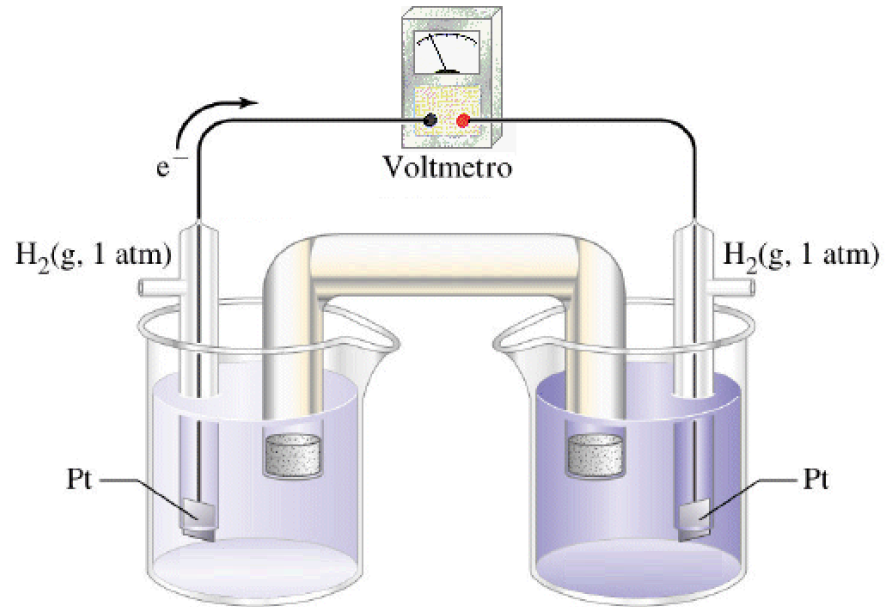
\includegraphics[width=12cm]{immagini/elettrodo_pH.png}
\end{figure}

\vspace{-1cm}$$\hspace{0.5cm}a_{\text{H}_3\text{O}^+}= 1 \hspace{3cm} a_{\text{H}_3\text{O}^+}=x<1$$

La d.d.p. sarà

$$E = 0.059 \log \frac{a'_{\text{H}_3\text{O}^+}}{a_{\text{H}_3\text{O}^+}}, \quad a'_{\text{H}_3\text{O}^+}=1 \implies E = 0.059 \log \frac{1}{a_{\text{H}_3\text{O}^+}}$$

$$ \implies E= 0.059 \, \text{pH} \implies \text{pH} = \frac{E}{0.059}$$


